%%%%%%%%%%%%%%%%%%%%%
%   AMS packages    %
%%%%%%%%%%%%%%%%%%%%%
\documentclass{amsart}

\usepackage{amsmath}
\usepackage{amsxtra}
\usepackage{amscd}
\usepackage{amsthm}
\usepackage{amsfonts}
\usepackage{amssymb}
\usepackage{eucal}
\usepackage[all]{xy}
\usepackage{graphicx}
\usepackage{tikz-cd}
\usepackage{mathrsfs}
\usepackage{subfiles}
\usepackage{euler}
\usepackage{hyperref}
\usepackage{color}
\usepackage{longtable}
\usepackage{float}
\usepackage{caption}
\usepackage{thmtools}
\usepackage{thm-restate}

\usepackage[colorinlistoftodos, textsize=tiny]{todonotes}
\def\listtodoname{List of Todos}
\def\listoftodos{\@starttoc{tdo}\listtodoname}

%\addtolength{\oddsidemargin}{-.5 in}
	%\addtolength{\evensidemargin}{-.4 in}
	%\addtolength{\textwidth}{1 in}
%
	%\addtolength{\topmargin}{0 in}
	%\addtolength{\textheight}{0 in}

\RequirePackage{color}
\definecolor{myred}{rgb}{0.75,0,0}
\definecolor{mygreen}{rgb}{0,0.5,0}
\definecolor{myblue}{rgb}{0,0,0.65}

%\usepackage{hyperref}
  %\hypersetup{colorlinks=true,citecolor=blue}

\usepackage{tikz}
\usepackage{tikz-cd}
\usetikzlibrary{matrix,arrows,decorations.pathmorphing}

%%%%%%%%%%%%%%%%%%%%%%% amsthm theorem styles %%%%%%%%%%%%%%%%%%%%%%%

\theoremstyle{plain}
  \newtheorem{thm}{Theorem}[section]
  \newtheorem{prop}[thm]{Proposition}
  \newtheorem{lem}[thm]{Lemma}
  \newtheorem{cor}[thm]{Corollary}
	\newtheorem{claim}[thm]{Claim}
	\newtheorem{question}[thm]{Question}
	
\theoremstyle{definition}
  \newtheorem{defn}[thm]{Definition}
  \newtheorem{example}[thm]{Example}
  \newtheorem{exer}[thm]{Exercise}
  \newtheorem{ctexample}[thm]{Counterexample}
  \newtheorem{convention}[thm]{Convention}
	\newtheorem{conjecture}[thm]{Conjecture}
	
\theoremstyle{remark}
	\newtheorem{rem}[thm]{Remark}
  \newtheorem{note}[thm]{Notation}
  \newtheorem*{note*}{Notation}
  \newtheorem{case}{Case}
	
\numberwithin{equation}{section}

%%%%%%%%%%%%%%%%%%%%%%%%% custom commands %%%%%%%%%%%%%%%%%%%%%%%%%%%

\newcommand\nc{\newcommand}
\nc\on{\operatorname}
\nc\renc{\renewcommand}
\newcommand\ssec{\subsection}
\newcommand\sssec{\subsubsection}
\newcommand\bh{{\mathbb H}}
\newcommand\bn{{\mathbb N}}
\newcommand\bc{{\mathbb C}}
\newcommand\bbf{{\mathbb F}}
\newcommand\br{{\mathbb R}}
\newcommand\bq{{\mathbb Q}}
\newcommand\bp{{\mathbb P}}
\newcommand\bz{{\mathbb Z}}
\newcommand\ba{{\mathbb A}}
\newcommand\bk{{\Bbbk}}

\newcommand\sco{{\mathscr O}}

\newcommand{\id}{\mathrm{id}}
\newcommand\im{\text{im }}
\newcommand\coker{\text{coker}}
\newcommand\gal{\mathrm{Gal}}

\DeclareMathOperator{\ord}{ord}
\DeclareMathOperator{\sym}{Sym}

%%%%%%%%%%%%%%%%%%%%% csurfaces custom commands %%%%%%%%%%%%%%%%%%%%%%%%%

\DeclareMathOperator\di{Div}
\newcommand\bida{a}
\newcommand\bidb{b}
\newcommand\pdeg{\delta}
\newcommand\hirz{\mathbb{F}}
\newcommand\mss{\mathscr{S}}

\DeclareMathOperator{\fr}{frac}
\DeclareMathOperator{\supp}{Supp}
\DeclareMathOperator{\initial}{in_\prec}
\DeclareMathOperator{\gin}{gin}
\DeclareMathOperator{\Eff}{Eff}
\DeclareMathOperator{\sat}{sat}
\DeclareMathOperator{\newspan}{span}
\DeclareMathOperator{\proj}{Proj}
\DeclareMathOperator{\spec}{Spec}
\DeclareMathOperator{\Te}{T_=}
\DeclareMathOperator{\Tp}{T_+}
\DeclareMathOperator{\Tm}{T_-}
\DeclareMathOperator{\num}{p}
\DeclareMathOperator{\den}{q}
\DeclareMathOperator{\lcm}{lcm}
\DeclareMathOperator{\Pic}{Pic}
%\captionsetup[table]{belowskip = 4pt}

\makeatletter
\newcommand{\customlabel}[2]{%
   \protected@write \@auxout {}{\string \newlabel {#1}{{#2}{\thepage}{#2}{#1}{}} }%
   \hypertarget{#1}{#2}
}
\makeatother

%%%%%%%%%%%%%%%%%%%%%%%%%%%%%% title %%%%%%%%%%%%%%%%%%%%%%%%%%%%%%%%

\title{Canonical rings of $\bq$-divisors on Minimal Rational Surfaces}

\author{Aaron Landesman}
\address[Aaron Landesman]{Department of Mathematics, Harvard University}
\email{aaronlandesman@college.harvard.edu}

\author{Peter Ruhm}
\address[Peter Ruhm]{Department of Mathematics, Stanford University}
\email{pruhm@stanford.edu}

\author{Robin Zhang}
\address[Robin Zhang]{Department of Mathematics, Stanford University}
\email{robinz16@stanford.edu}

\date{\today}

%%%%%%%%%%%%%%%%%%%%%%%%%%%%% document %%%%%%%%%%%%%%%%%%%%%%%%%%%%%%

\begin{document}
\begin{abstract}
 	We give bounds on the degree of generation and relations of
	canonical rings of arbitrary $\bq$-divisors
	on projective spaces of all dimensions
	and Hirzebruch surfaces. We also give an explicit presentation 		and tight bounds on the
	generators and relations of the canonical ring of effective
	stacky divisors on projective spaces of any dimensions.
\end{abstract}

\maketitle

%%%%%%%%%%%%%%%%%%%%%%%%%%%% Introduction %%%%%%%%%%%%%%%%%%%%%%%%%%%%%%%

\section{Introduction}
\label{sec:intro}
For any Weil $\bq$-divisor $D$ on a rational surface $X$, the graded
\textbf{canonical ring} is $R(X, D) := \bigoplus_{d \geq 0} u^d H^0(X, \lfloor dD \rfloor)$, where $u$ is a dummy variable to keep
track of degree.
We study the generators and relations of canonical
rings for projective spaces $\bp^m$ and Hirzebruch surfaces $\hirz_m$.
When $D$ is a general $\bq$-divisor on $\bp^m$ or
$\hirz_m$, we give bounds on the generators and relations of
$R(X, D)$. In particular, we give a minimal presentation of the
canonical ring when $X = \bp^m$ and $D$ is any effective
$\bq$-divisor.  

In part, this work is motivated by a recent paper by
O'Dorney \cite{dorney:canonical}, which gives similar descriptions
of canonical rings for general $\bq$-divisors on $\bp^1$. This
study also has connections to the papers by Voight--Zureick-Brown 
\cite{vzb:stacky} and Landesman--Ruhm--Zhang \cite{lrz:spin-cring},
which provide tight bounds on generators and relations
of canonical rings and spin canonical rings, respectively, on arbitrary stacky curves.

Another closely related topic is the Hassett-Keel program \cite{hassett:classical-and-minimal-models}, which aims to describe log canonical models of the form 
\begin{align*}
	\overline {\mathscr M}_g(\alpha) := \bigoplus_{d \geq 0} u^d H^0 \left(
	\overline {\mathscr M}_g, \lfloor d K_{\overline{\mathscr M}_g} +
	\alpha\delta \rfloor  \right) 
\end{align*}
in terms of certain moduli spaces, where $\overline {\mathscr M_g}$ is the
moduli space of stable genus $g$ curves.
Moreover, $\bq$-divisors on surfaces also naturally
appear when considering the canonical ring of surfaces of Kodaira dimension 1.
A surface has Kodaira dimension 1 if and only if it is an elliptic surface \cite[p. 244]{
barthHPV:compactComplexSurfaces}, and
the canonical rings of elliptic surfaces most naturally described in the setting of
$\bq$-divisors \cite[Chapter V, Theorem 12.1]{barthHPV:compactComplexSurfaces}. 

We expect the work in this paper will help calculate a presentation of certain rings of
Hilbert 
modular forms and Siegel modular forms. Recall that Hilbert and Siegel 
modular forms are two generalizations of modular forms to higher dimensions,
as described in \cite{geer:siegel-modular} and \cite{bruinier:hilbert-modular}.
Voight and Zureick-Brown show that 
one can translate the analytic category of 1-dimensional complex orbifolds to
the algebraic category of stacky curves \cite[Proposition 6.1.5]{vzb:stacky}. 
We expect that one can generalize this result to yield an equivalence of
categories between an appropriate subcategory of $m$-dimensional orbifolds and
a subcategory of $m$-dimensional algebraic spaces.
In particular, this would allow us to translate rings of Hilbert modular forms
and Siegel modular forms whose coarse space is a projective space or a
Hirzebruch surface to canonical rings on the corresponding algebraic surfaces.
Thereby, our techniques would give a bound on generators and relations for such
Hilbert and Siegel modular forms.

\ssec{Main Results and Outline}

In Section \ref{sec:proj} we prove the following two results bounding
the degree of generators and relations of
stacky canonical rings on $\bp^m$:
\begin{restatable}{thm}{restateeffective}
\label{thm:proj-effective-intro}
Let $D = \sum_{i = 0}^{n} \alpha_i D_i \in \bz \otimes_\bz \di \bp^m$, with $\alpha_i =
\frac{c_i}{k_i} \in \bq_{> 0}$ and let each $D_i$ be a hypersurface of
$\bp^m$.

Then the canonical ring
\[
	R_D := \bigoplus_{d \geq 0} u^d H^0(\bp^m, \lfloor dD \rfloor)
\]

\noindent
is generated in degrees at most $\max_{1 \leq i \leq n}{k_i}$ with
relations generated in degrees at most $2 \max_{1 \leq i \leq n}{k_i}$
\end{restatable}

\begin{restatable}{thm}{restateproj}
\label{thm:proj-generators-relations}
Let $\bp^m$ have projective coordinates $x_0,\ldots, x_m$. Let $D = \sum_{i=0}^n \alpha_i D_i \in \bq \otimes_\bz \di \bp^m$ where $\alpha_i = \frac{c_i}{k_i}$.
Then notate \todo{Peter: It seems a bit weird to me how we define this notation.  It is used throughout the paper and defined here, but after this point it is never redefined nor is it referenced to this definition.  Would it be good to make this into an equation and reference the first time it is used in section 2?}
\[\ell_i = \lcm_{j\ne i}(k_j).\] 
Let
$f_0, \ldots, f_n$ be homogeneous polynomials in $x_0, \ldots, x_m$ such that
$D_i = V(f_i)$ for all $i$, $\deg(f_i) = a_i,$ and $f_0,\ldots, f_m$ are independent linear polynomials in $x_0, \ldots, x_m$. 
Then $R_D$ is generated in degrees at most 
\[
	\sum_{i=0}^n \ell_i a_i
\]

\noindent
with relations generated in degrees at most
\[
	\max \left(2 \sum_{i=0}^n \ell_i a_i, \frac{\max_{0\le i \le n}
	(	\bida_i)}{\deg(D)} + \sum_{i=0}^n \ell_i a_i \right).
\]
\end{restatable}

\noindent
In Section \ref{sec:hirz}, we shift our attention to Hirzebruch Surfaces and prove the following theorem:
\begin{restatable}{thm}{hirzrestate}
\label{thm:hirz-generators-relations}
Let $u,v,z,w$ be the coordinates for the Hirzebruch surface $\hirz_m$, as described at the beginning of Section ~\ref{sec:hirz}. Let $D = \sum_{i=1}^n \alpha_i D_i \in \bq \otimes_\bq \di \hirz_m$ 
where $\alpha_i = \frac{c_i}{k_i}$.
Then notate \todo{Peter: Same comment as above.}
\[\ell_{i,j} = \lcm_{h\ne i,j}(k_h).\] 
Let $D_i =
V(f_i)$ where $f_i \in \sco(a_i, b_i)$; further suppose $f_1$ and $f_2$ are
independent linear
polynomials in $u$ and $v$ and $f_3$ and $f_4$ are independent
linear polynomials in $w$ and $x$.
Then $R_D$ is generated in degrees at most
\[
	\rho = \sum_{i\in \Te(D)} \gcd(\bida_i, \bidb_i)\ell_i +
	\sum_{\substack{i \in \Tp(D) \\	j \in \Tm(D)}} (\bida_i \bidb_j
	- \bida_j \bidb_i) \ell_{i, j}
\]

\noindent
with relations generated in degrees at most 
\[
	\max(2 \rho, \tau)
\]

\noindent
where
\[
	\tau = \rho
	+ \max \left( \max_{i\in \Te} \bigl(\ell_i \gcd(a_i, b_i) \bigr),
	\max_{\substack{i \in \Tp \\ j \in \Tm}} \bigl(\ell_{i, j}
	(\bida_i \bidb_j - \bida_j \bidb_i) \bigr) \right).
\]
\end{restatable}

\noindent
Together, Theorems \ref{thm:proj-generators-relations} and \ref{thm:hirz-generators-relations} provide bounds on generators and relations for the canonical ring of $\bq$-divisors of all minimal rational surfaces.  Section \ref{sec:conc} concludes the paper and discusses further questions.

\ssec{Notations and Conventions}
Notate a (Weil) $\bq$-divisor
\begin{align*}
	D = \sum_{i=1}^{n}\alpha_i D_i \in \di X \otimes \bq.
\end{align*}

\noindent
where $\alpha_i \in \bq$ and $D_i \in \di X$ is an integral codimension 1 closed subscheme of $X$. When it is convenient to do so, we shall sometimes start the indexing at $0$, so that $i$ runs from $0$ to $n$. The degree of $D$ is by definition $\deg D = \sum_{i=1}^{n}\alpha_i$. For such a divisor $D$ with $\alpha_i = \frac{c_i}{k_i}$ let $\ell_i = \lcm_{j\ne i}(k_j)$
and let $\ell_{i,j} = \lcm_{h\ne i,j}(k_h).$ The floor of a $\bq$-divisor $D$ is a divisor $\lfloor D
\rfloor \in \di X$ is defined to be $\lfloor D \rfloor := \sum_{i = 1}^{n}
\lfloor \alpha_i \rfloor P_i$. Let $
	R_D := \bigoplus_{d \geq 0} u^d H^0(\bp^m, \lfloor dD \rfloor)$
denote the canonical ring associated to the $\bq$-divisor $D$. If $R$
is a graded ring, we denote the $d$th graded component of $R$ by $R_d$. If $r$ is a rational number, we let
$\fr(r) := r - \lfloor r
\rfloor$ denote the fractional part of $r$.
\section{Canonical Rings on Projective Space}
\label{sec:proj}
In this section, we bound the degrees of generators and relations for divisors
on $\bp^m$, for all $m \geq 1$ in Theorem ~\ref{thm:proj-effective-intro}. 
The $\bp^1$ case restricts to the results of
\cite{dorney:canonical}. We also give an explicit description of the
generators of the canonical ring $R_D$ when $D$ is an effective divisor in Theorem ~\ref{thm:proj-generators-relations}


For the remainder of this section, we shall fix $m \geq 1$ and choose an
isomorphism $\bp^m \cong \proj V$ for some vector space $V$ with basis $x_0,\ldots, x_m$.  We will think of $x_i$ as a rational section of $H^0(\bp^m,
\sco_{\bp^m})$ of degree 1.

\ssec{Preliminaries on Projective Space}
Before bounding the degree of generation and relations of
canonical rings on projective space, we first
describe a particular choice of basis for $R_D$ as a $\bk$ vector space.

Write
\begin{align*}
	D = \sum_{i=0}^{n}\alpha_i D_i.
\end{align*}
where $n \in \bz$, $\alpha_i \in \bq$, and $\deg D_i = \bida_i$. Let $D_i$ be
Cartier divisors such that $D_i = V(f_i)$.
We shall further assume for this subsection that (possibly after reordering) $f_0,\ldots, f_{m}$ form a
basis for degree one rational functions on $\bp^m$.  

\begin{prop}
\label{prop:pm-span-and-basis}
The functions $u^d \cdot \prod_{i=1}^n f_i^{c_i} \in (R_D)_d$ satisfying

\begin{align}
\label{align:pm-span}
\sum_{i=0}^{n} c_i \cdot \bida_i = 0 && \text{ and } &&c_i \geq \lfloor \alpha_i d\rfloor	
\end{align}

\noindent
form a spanning set for $H^0(\bp^m, dD)$ over $k$. Furthermore, functions 
of the form $u^d \cdot \prod_{i=0}^n f_i^{c_i}$ satisfying
\begin{align}
\label{align:pm-basis}
c_i = -\lfloor d\alpha_i \rfloor && \text{ for } && i > m
\end{align}

\noindent
form a basis for $H^0(\bp^m, dD)$ over $k$.
\end{prop}

\begin{proof}
By definition of $H^0(\bp^m,dD)$, functions satisfying conditions 
~\eqref{align:pm-span} lie in $H^0(\bp^m,dD)$. To complete the proof, it
suffices to check functions satisfying conditions ~\eqref{align:pm-basis} form
a basis of $H^0(\bp^m,dD)$. Note that there $\binom{m+ \lfloor dD \rfloor }{m}$
functions satisfying condition ~\eqref{align:pm-basis}. However we know
$h^0(\bp^m,dD) = \binom{m+ \lfloor dD \rfloor }{m},$ so it suffices to show
that those functions satisfying condition ~\eqref{align:pm-basis} are
independent. This follows from the assumption that $f_0,\ldots f_n$ form a
basis of degree 1 rational functions, and so all monomials in $f_0,\ldots, f_m$ of degree degree $\lfloor d \deg D \rfloor $
form a basis of degree $\lfloor d \deg D \rfloor$ rational functions.
\end{proof}

\ssec{Effective Divisors on Projective Space}
\label{ssec:proj-one-point}

In this subsection, we restrict attention to the case of effective
fractional divisors $D \in \bq \otimes \di \bp^m$. We give an explicit presentation of the canonical ring when $D$ is an effective
divisor.

\begin{convention}
Let $[x_0, \ldots, x_m]$ be coordinates for $\bp^m$. Let
$\vec{v} = (v_0, \ldots, v_m) \in \bz^{m + 1}$.  Then write
\[
	x^{\vec{v}} := \prod_{i = 0}^{m} x_i^{v_i}.
\]
\end{convention}

\begin{defn}
\label{defn:vec-sum}
For $\vec{v} \in \bz^n$, denote $\deg \vec{v} := \sum_{i = 0}
^n v_i$.
Let 
\begin{align*}
	\mss_i := \left \{\vec{v} \in \bz_{\geq 0}^{m + 1} \; : \;
\deg \vec v = c_i \right\}.	
\end{align*}

\noindent
\end{defn}

Next, we define an ordering on these vectors, which will be used to give a presentation for $R_D$. Although it is not
stated explicitly later, in the case that $D = \alpha_1 D_1$ is supported on a single hypersurface, the relations in
Theorem ~\ref{thm:proj-one-point} form a reduced grobner basis with respect to
this ordering.

\begin{defn}
\label{defn:vec-order}
Let $\vec{v}, \vec{w} \in \bz^{m+1}$. Let $i \in \{0,\ldots, m\}$
be the biggest index such that $v_i$ is nonzero
and $j \in \{0,\ldots, m\}$ be the smallest index such that $w_j$ is
nonzero. Define a partial ordering on $\bz^{m+1}$ by $\vec{v} \prec \vec{w}$ if $i \leq j$.
\end{defn}

We are now ready to give an inductive method for computing
the generators and relations of $R_D$ in terms of $R_{D'}$ 
in the case that $D' = R_D + \alpha H$ for $H$ a hyperplane.
The statement and proofs are natural generalizations of
\cite[Theorem 6]{dorney:canonical}.


\begin{thm}
\label{thm:proj-one-point}
Let $\bp^m \cong \proj \bk [x_0, \ldots, x_m].$ Let $D' \in \bq
\otimes \di \bp^m$ and $D = D' + \alpha H$, with $\alpha =
\frac{p}{q} \in \bq$ and $H := V(x_k)$ a hyperplane of $\bp^m$.
Let
\[
	0 = \frac{c_0}{d_0} <
	\frac{c_1}{d_1} < \ldots < \frac{c_r}{d_r} = \frac{p}{q}
\]

\noindent
be the best lower approximations of $\alpha$. Then, the
canonical ring
\[
	R_D := \bigoplus_{d \geq 0} u^d H^0(\bp^m, \lfloor dD \rfloor)
\]

\noindent
has a minimal presentation over $R_{D'}$ consisting of the $\sum_{i = 0}^{r}
{{m + c_i - 1} \choose {c_i}}$ generators $F_i^{\vec{v}} := \frac{u^{d_i}
x^{\vec{v}}}{x_k^{c_i}}$ where $1 \leq i \leq r$, $\vec{v} \in \bz_{\geq 0}^{m + 1}$
with $\deg \vec v = c_i$. Furthermore, it has
relations generated by the following two classes of elements.
\begin{enumerate}
	\item For each $(i, j)$ with $j \geq i + 2$ and each $\vec{v} \in \mss_i,
\vec{w} \in \mss_j$, there is a relation of the form either
\begin{flalign*}
	&G_{i, j}^{\vec{v}, \vec{w}} = F_i^{\vec{v}} F_j^{\vec{w}}
	- \prod_{\vec{y} \in \mss_{h_{i, j}}} (F_{h_{i, j}}^{\vec{y}})
	^{g_{\vec{y}}} &(i < h_{i, j} < j) \\
	\text{or} \\
	&G_{i, j}^{\vec{v}, \vec{w}} = F_i^{\vec{v}} F_j^{\vec{w}}
	- \prod_{\vec{y} \in \mss_{h_{i, j}}} (F_{h_{i, j}}^{\vec{y}})^{g_{\vec{y}}}
	\cdot \prod_{ \vec{z} \in
	\mss_{h_{i, j} + 1}} (F_{k_{i, j} + 1}^{\vec{z}})^{g'_{\vec{z}}}
	&(i < h_{i, j} < h_{i, j} + 1 < j).
\end{flalign*}
	\item For each $(i, j)$ with
$j = i$ or $j = i + 1$ and each $\vec{v} \in \mss_i, \vec{w} \in
\mss_j$ with $\vec{v} \not\prec \vec{w}$ (see Definition
~\ref{defn:vec-order}) there is a relation of the form
\begin{align*}
	&L_{i, j}^{\vec{v}, \vec{w}} = F_i^{\vec{v}} F_j^{\vec{w}}
	- F_i^{\vec{y}} F_j^{\vec{z}} \\
\end{align*}

\end{enumerate}

\noindent
where $\vec{y}$ and $\vec{z}$ are the unique
vectors in $\mss_i$ and $\mss_j$, respectively, such that $\vec{y}
+ \vec{z} = \vec{v} + \vec{w}$ and $\vec{y} \prec \vec{z}$.
\end{thm}

\sssec*{Idea of Proof:}
The proof follows in four steps. First, we demonstrate that
the $F_{i}^{\vec{v}}$'s form a set of minimal generators of $R_D$
over $R_{D'}$ using their construction in terms of best lower
approximations to $\alpha$. Then, since the $F_{i}^{\vec{v}}$ generate
all of $R_D$ over $R_{D'}$, we obtain the
relations $G_{i, j}^{\vec{v}, \vec{w}}$.
We derive the relations
$L_{i, j}^{\vec{v}, \vec{w}}$ by considering when products of
generators in neighboring degrees are equal. Finally, we demonstrate
that $G_{i, j}^{\vec{v}, \vec{w}}$'s and $L_{i, j}^{\vec{v}, \vec{w}}$'s
generate all of the relations by using them to reduce arbitrary
elements of
$R_D$ to a canonical form.

\begin{proof}
For simplicity, we give a proof for when $D' = 0$, but the general
can be analogously proved by replacing the orders of zeros and poles
by the order of zeros and poles relative to $D'$. That is,
one can work with rational sections of $\mathscr O_{\bp^m}(D')$
instead of rational sections of $\mathscr O_{\bp^m}$,
and the following proof goes through otherwise unchanged.

We will first check that $F^{\vec v}_i$ determine a system of minimal
generators of $R_D$. We know $\left\{F_{1}^{\vec{v}} : \deg \vec{v} =
\left\lfloor
\frac{p}{q} \right\rfloor \right\}$ are minimal generators in
degree $1$. Now let $i > 1$. Suppose $F_i^{\vec{v}}$ were not
minimal for some $\vec{v} \in \mss_i$. Then $F_i^{\vec{v}} =
F_{s}^{\vec{y}} F_{t}^{\vec{z}}$ for some $s, t \in \bn$ and
$\vec{y}, \vec{z} \in \bz_{ \geq 0}^{m + 1}$. In particular, we see
that 
\begin{align*}
	&d_i = s + t \\
	&c_i = \deg \vec{v} = \deg \vec{y} + \deg \vec{z}
\end{align*}

\noindent
so $\frac{c_i}{d_i}$ is the mediant of the rational numbers
$\frac{\deg \vec{y}}{s}, \frac{\deg \vec{z}}{t}$ which both
do not exceed $\alpha$. One of $\frac{\deg \vec{y}}{s},
\frac{\deg \vec{z}}{t}$ must be at least $\frac{c_i}{d_i}$
and $s$ and $t$ are both less than $d_i$, which contradicts the assumption that
$\frac{c_i}{d_i}$ is a best lower approximation of $\alpha$
(see Definition ~\ref{defn:lower-approximation}). Therefore, none of the $F_i^{\vec v}$ are redundant.

Next we show that $F^{\vec v}_i$ generate all of $R_D$. In the case $m = 1$, O'Dorney \cite[Theorem 6]
{dorney:canonical} demonstrates that each lattice point $(\beta, \gamma) \in
\bz_{\geq 0}^2$ with $\gamma \leq \beta \alpha$ lies in the $\bz_{\geq 0}$ span
of $(d_h, c_h)$ and $(d_{h + 1}, c_{h + 1})$ for
some $h \in \{0, \ldots, r\}$. A similar strategy works in the case $m > 1$. Let $(\beta, \gamma) = \kappa_1
(d_h, c_h) + \kappa_2 (d_{h + 1}, c_{h + 1})$ for $\kappa_1, \kappa_2 \in
\bz_{\geq 0}$. Any element $\frac{u^{\beta}
x^{\vec{v}}} {x_k^{ \gamma}} \in R_D$ is expressible as
\begin{align*}
	\frac{u^{\beta} x^{\vec{v}}} {x_k^{\gamma}} = \left(\frac{u^{d_h}}
	{x_k^{c_h}}\right)^{\kappa_1} \left(\frac{u^{d_{h + 1}}}
	{x_k^{c_{h + 1}}}\right)^{\kappa_2} x^{\vec{v}}.
\end{align*}

\noindent
We can then write $\vec{v}  = \sum_{\lambda=1}^{\kappa_1}\vec{w}_{(\lambda)} +
\sum_{\eta=1}^{\kappa_2} \vec z_{(\eta)}$ with $w_{(\lambda)} \in \mss_h$ and
$z_{(\eta)} \in \mss_{h+1}$ to give a decomposition
\begin{align}
\label{eqn:one-point-canonical-form}
	\frac{u^{\beta} x^{\vec{v}}} {x_k^{\gamma}}	= \prod_{\lambda = 1}
	^{\kappa_1} \frac{u^{d_h} x^{\vec{w}_{(\lambda)}}} {x_k^{c_h}}
	\prod_{\eta = 1}^{\kappa_2} \frac{u^{d_{h + 1}} x^{\vec{z}_{(\eta)}}}
	{x_k^{c_{h + 1}}}
\end{align}
\noindent
consisting of products of generators $F_h^{\vec{y}_{(\lambda)}}$
and $F_{h + 1}^{\vec{z}_{(\eta)}}$ which are in the form
prescribed in the theorem statement. Since we wrote an arbitrary monomial
$\frac{u^{\beta} x^{\vec{v}}}{x_k^\gamma} \in R_D$ as a product of generators,
this shows that $F_i^{\vec v}$ minimally generate $R_D$.

Next, we show that the relations given in the statement of the theorem generate all relations. 
In particular, if $j \geq i + 2$ then $F_i^{\vec{v}} F_j^{\vec{w}}$
has a decomposition of the form ~\eqref{eqn:one-point-canonical-form} of 
products of generators in adjacent degrees where $h$
depends on $i$ and $ j$, so we notate $h_{i, j} := h \in \{1, \ldots, r\}$. We 
also have that $i \leq h_{i, j} < j$ since $(d_i + d_j, c_i + c_j)$ is in the
$\bz_{\geq 0}$-span of $(d_{h_{i, j}}, c_{h_{i, j}})$ and
$(d_{h_{i, j} + 1}, c_{h_{i, j} + 1})$. Furthermore,
$h_{i, j} \neq i$ and $h_{i, j} \neq j - 1$
as follows from an analogous proof to that given by O'Dorney
\cite[Theorem 6]{dorney:canonical} for the case of
$\bp^1$. This gives the relations
$G_{i, j}^{\vec{v}, \vec{w}}$.

One can use the relations $G_{i, j}^{\vec{v}, \vec{w}}$
to transform any monomial in the $F_i^{\vec{v}}$'s involving
indices that differ by more than $1$ to a monomial in the $F_i
^{\vec{v}}$'s involving indices that differ by at most $1$.

We also have relations involving generators in consecutive
indices. Suppose $F_i^{\vec{v}}$ and $F_j^{\vec{w}}$ are
generators with $j = i$ or $j = i + 1$ and $\vec{v} \in
\mss_i, \vec{w} \in \mss_j$ with $\vec{v} \not\prec \vec{w}$.
Let $\vec{y}$ and $\vec{z}$ be the unique vectors in $\mss_i$ and
$\mss_j$, respectively, such that $\vec{y} + \vec{z} = \vec{v} +
\vec{w}$ and $\vec{y} \prec \vec{z}$ (i.e.~ the nonzero indices
of $\vec{y}$ followed by those of $\vec{z}$ give an increasing
sequence). Then we see that
\begin{align*}
	F_i^{\vec{v}} F_j^{\vec{w}} = x^{\vec{v} + \vec{w}}
	\left(\frac{u^{d_i}}{x_k^{c_i}}\right)
	\left(\frac{u^{d_j}}{x_k^{c_j}}\right)
	= x^{\vec{y} + \vec{z}}
	\left(\frac{u^{d_i}}{x_k^{c_i}}\right)
	\left(\frac{u^{d_j}}{x_k^{c_j}}\right)
	= F_i^{\vec{y}} F_j^{\vec{z}},
\end{align*}

\noindent 
which give the relations $L_{i, j}^{\vec{v}, \vec{w}}$.

Now, we may apply the relations $L_{i, j}^{\vec{v}, \vec{w}}$
to any monomial in the $F_i^{\vec{v}}$'s involving
indices that differ by at most $1$ to produce the canonical form
\begin{align*}
	(F_i^{\vec{v}_{(1)}})^{g_{\vec{v}_{(1)}}} \cdots
	(F_i^{\vec{v}_{(\kappa_1)}})^{g_{\vec{v}_{(\kappa_1)}}}
	(F_{i + 1}^{\vec{w}_{(1)}})^{g_{\vec{w}_{(1)}}} \cdots
	(F_{i + 1}^{\vec{w}_{(\kappa_2)}})^{g_{\vec{w}_{(\kappa_2)}}}
\end{align*}

\noindent
where $\vec{v}_{(1)} \prec \vec{v}_{(2)} \prec \ldots \prec
\vec{v}_{(\kappa_1)} \prec \vec{w}_{(1)} \prec \ldots \prec
\vec{w}_{(\kappa_2)}$. Consequently, the relations of form
$G_{i, j}^{\vec{v}, \vec{w}}$ and of form $L_{i, j}^{\vec{v},
\vec{w}}$ generate all the relations among the $F_{i}^{\vec{v},
\vec{w}}$.
\end{proof}

\begin{rem}
\label{rem:proj-two-points}
Note that we cannot extend this result to the case when
$D$ is supported at two hypersurfaces with arbitrary rational (non-effective)
coefficients in the same manner that O'Dorney does for the
$\bp^1$ case \cite[Section 4]{dorney:canonical}. As will be shown
in Example ~\ref{eg:hyperplane}, the degrees of generation of the
canonical ring of a general $\bq$-divisor supported on two
hyperplanes cannot be bounded so tightly. The two-point
$\bp^1$ result leverages the fact that $\bp^1$ has precisely two
independent coordinates, so that two distinct integral subschemes
cannot be equations of only $m$ of the $m+1$ coordinates.
\end{rem}

%\begin{rem}
%\label{rem:proj-one-point-ind}
%The method of proof for Theorem ~\ref{thm:proj-one-point}
%can be immediately generalized to work inductively. If $D = D' + \alpha H$
%for some hyperplane $H$, then the proof of Theorem ~\ref{thm:proj-one-point}, mutatis mutandis, extends to show
%the canonical ring $R_D$ is generated over $R_D'$ by the same
%generators and with the same relations given in Theorem
%~\ref{thm:proj-one-point}.
%\end{rem}

Theorem ~\ref{thm:proj-one-point} gives an inductive procedure to
compute presentations of effective divisors which are supported on
hyperplanes. However, for $m \geq 2$, there are hypersurfaces which
are not unions of hyperplanes. We now address this general case, giving an inductive presentation of canonical rings of effective divisors, and a tight bound on the degrees of their generators and
relations.

\restateeffective*


\begin{proof}
We proceed by induction on $n$.
If $n = 0$, i.e.~ $D = 0$, then we are done.
Now, we inductively add hypersurfaces.
Let $D' = \sum_{i = 0}^{n} \alpha_i D_i \in \bq \otimes_\bq\di \bp^m$, 
and assume the theorem holds for $D'$. It suffices to show
the theorem holds for $D \in \di \bq \otimes_\bq \bp^m$, where $D = D' + \alpha C$ for some
degree $\pdeg$ hypersurface $C$.
If $C$ were a hyperplane, we would then be done, by Theorem ~\ref{thm:proj-one-point}.

To complete the theorem, we reduce the case that $C$ is a general hypersurface
to the case that $C$ is a hyperplane, by using the Veronese embedding.

If $C$ is of degree $\pdeg$, consider the Veronese embedding
$\nu_\pdeg^m: \bp^m \rightarrow \bp^{\binom{m+\pdeg}{\pdeg}-1}$
so that the image of $C$ is the intersection of 
a hyperplane in $\bp^{\binom{{m + \pdeg}}{\pdeg} - 1}$ with $\nu_\pdeg^m(\bp^m)$.
Now, note that the ring $R_{\alpha C}$ is isomorphic to the
$\pdeg$ Veronese subring of $R_{\alpha V(x_0)} = \bigoplus_{d \geq 0} u^d H^0(\bp^m, d \alpha V(x_0))$ and so
the canonical ring $R_H$ of the hyperplane $H \subset \bp^{\binom{m+\pdeg}{\pdeg}-1}$
restricted to $\nu_\pdeg^m(C)$ is isomorphic to $R_C$.
Therefore, we can bound the degree of generators and relations of
$R_D$ over $R_{D'}$ by the degree of generators and
relations for $R_C \cong R_H.$
This reduces the case of a hypersurface $C$ to
a hyperplane $H$, completing the proof by Theorem
~\ref{thm:proj-one-point}.
\end{proof}

\begin{rem}
\label{rem:exact-effective-bounds}
Note that the proof of Theorem ~\ref{thm:proj-effective-intro} not only gives bounds on the degrees of the generators and relations, but actually gives an explicit method for computing the presentation. In particular, these bounds are tight. The generator bound is always achieved and the bound on the relations is achieved if $m \geq 2$.
\end{rem}



\ssec{Bounds for Arbitrary Divisors on Projective Space}


We now offer bounds on generators and relations of $R_D$ for a general $\bq$-divisor $D \in \bq \otimes_\bq \di \bp^m$.

Let $D = \sum_{i=0}^n \alpha_i D_i \in \bq \otimes \di \bp^m$ and let $f_i$ be
homogeneous polynomials in $x_0, \ldots, x_m$ such that $D_i = V(f_i)$
$\deg(f_i) = a_i$ for all $i$. 

For the remainder of this section, we shall make the additional assumption that 
\begin{align} \label{eqn:pm-basis-assumption} f_0, \ldots, f_{m} \text{ form a
	} \bk \text{ basis of all degree 1 functions.} \end{align}

The first aim of this section is to prove Theorem
~\ref{thm:proj-generators-relations} bounding the number of generators and
relations of $R_D$. Before doing so, we justify the importance of assumption
~\eqref{eqn:pm-basis-assumption} with several illustrative examples.

\begin{example}
\label{eg:hyperplane}
In this example,we show that the naive generalization of
~\cite[Theorem 8]{dorney:canonical} of generation in degree at most
$\sum_{i=0}^{n}\ell_i$ cannot possibly hold. The reason for this is
that the divisors may be
expressible as functions in $m$ of the $m+1$ variables on $\bp^m$.

Concretely, take $D = \frac{1}{2}H_0 - \frac{1}{3}H_1$ where $H_0 = V(x_0),
H_1 = V(x_1)$ are two coordinate hyperplanes in $\bp^2$. Then, $R_D$
has generators in degree $2$ and $3$ which can be written as $u^2
\frac{x_1}{x_0}, u^3 \frac{x_1}{x_0}.$ In fact, for all degrees
less than $5$, the elements of $R_D$ can all be expressed as
rational functions in $x_0, x_1$. However, in degree $6$, there is
$u^6 \frac{x_1^2 x_2}{x_0^3}$. Since this
involves $x_2$, it must be a generator.

This example generalizes slightly to any divisor of the form $D =
\frac{1}{k}H_0 - \frac{1}{k+1}H_1 \in \di \bp^2 \otimes \bq,$ with
$k \in \bn$, showing that there will always exist a generator in
degree $a(a + 1)$.

This example further generalizes to the following situation:
Suppose $D = \sum_{i=0}^{n} \frac{\num_i}{\den_i}D_i \in \di \bp^m
\otimes \bq,$ where $\deg D_i = \bida_i$ and $\deg D = \frac{1}{\lcm
_{0 \leq i \leq n}(\den_i \cdot \bida_i)}$. Then, if $D_i = V(f_i)$
where all $f_i$ can be written as a polynomial function in $x_0,
\ldots, x_{m-1},$ it follows that $R_D$ always has a generator in degree
$\lcm(\den_i \cdot \bida_i)$.
\end{example}

The problem that a divisor may be
expressible as functions in $m$ of the $m+1$ variables on $\bp^m$, 
as illustrated in Example ~\ref{eg:hyperplane}, can easily be circumvented by adding in ``ghost
points.'' That is, we may add divisors of the form $0 \cdot H_i$ to
$D$, and reorder so that if $D = \sum_{i=0}^{n}\alpha_i V(f_i)$,
then $f_0, \ldots, f_m$ are independent linear functions in
$x_0,\ldots, x_m$.

In Example ~\ref{eg:radical}, we show that it is still, in general,
necessary to add ghost points, even when the irreducible components
of a divisor are not all
expressible as functions in $m$ of the $m+1$ variables on $\bp^m$.

\begin{example}
\label{eg:radical}
Consider $\frac{-1}{5}V(x_0^2 + x_1^2 + x_2^2) + \frac{1}{7}V(x_0^2 + x_1^2 +
x_3^2) + \frac{1}{17}V(x_0^2 + x_2^2 + x_3^2) - \frac{1}{596}V(x_1^2 + x_2^2 +
x_3^2)$. In degree $355216 = 5 \cdot 7 \cdot 17 \cdot 596$, this has dimension
$6$.
However,  approach, as all lower degrees only have
dimension at most 1. Therefore, we cannot hope to bound the degree
of generation of $R_D$ as a linear combination of $\ell_i$,
in analogy to \cite[Theorem 8]{dorney:canonical}
unless we require that $D$ includes ghost points. That is, unless
$D_0,\ldots D_m$ are taken to be linearly independent hyperplanes.
\end{example}

Having justified the necessity of adding ghost points, we proceed to bound the
number of generators and relations of arbitrary $\bq$-divisors in 
projective space. We bound the generators in Lemma ~\ref{lem:proj-generators}, and we use Lemmas ~\ref{lem:composite-map}, ~\ref{lem:bound-ker-chi}, and ~\ref{lem:proj-relations-psi} to bound the 
degree of relations in the proof of Theorem ~\ref{thm:proj-generators-relations}. Note that Proposition ~\ref{prop:cone-generation}, Lemma ~\ref{lem:composite-map}, and Lemma ~\ref{lem:bound-ker-chi} are quite 
general and will also be used in Section ~\ref{sec:hirz} to bound the 
degree of generators and relations on Hirzebruch surfaces.

\begin{defn}
\label{defn:lower-approximation}
If $\alpha \in \bq$, then a rational number $\frac{c}{k} \leq \alpha$
(written in reduced form with $c \in \bz, k \in \bn$) is a
\textbf{best lower approximation} to $\alpha$ if there does not
exist $\frac{c'}{k'}\in \mathbf{Q}$ such that $0 < k'< k$ and
$\frac{c}{k} \le \frac{c'}{k'} \le \alpha$. 
\end{defn}

\begin{rem}
\label{rem:lower-approximation}
Note that all integers less than or equal to $\lfloor \alpha \rfloor$
are best lower approximations to $\alpha$. Also, if $\alpha \ge 0$,
then the non-negative best lower approximations of
$\alpha$ form a finite sequence
\[
	0 = \frac{c_0}{k_0} < \frac{c_1}{k_1} < \ldots < \frac{c_r}{k_r} = \alpha.
\]

\noindent
Figure ~\ref{fig:s14/5-lattice} gives a pictorial representation of the best lower approximations of $\alpha = \frac{14}{5}$.
\end{rem}

\begin{figure}
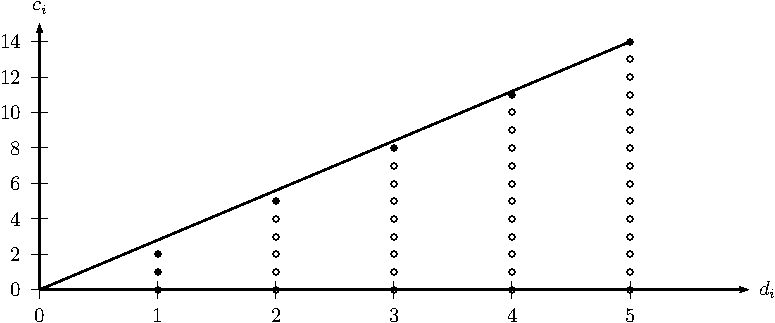
\includegraphics{pics/spin-lower-approximations-pic-pics.pdf}
\caption{This figure shows each non-negative best lower
approximation of $\frac{14}{5}.$ Each ``$\bullet$'' denotes a best
lower approximation and each ``$\circ$'' denotes a lattice point
below $5y=14x$ which is not a best lower approximation.  Note that
the non-negative best lower approximations generate the monoid of
lattice points in the first quadrant satisfying  $5y \le 14x$, with
the operation $(a_1, b_1)(a_2, b_2)\mapsto (a_1 + a_2, b_1 + b_2)$.}
\label{fig:s14/5-lattice}
\end{figure}

\begin{prop}
\label{prop:cone-generation}
Let $n \in \bz,$ let $\alpha_1, \ldots, \alpha_n \in \bq$, and let
$a_i, b_i \in \bz$ with $1 \leq i \leq n.$ Define
\begin{align*}
	\Sigma := \left \{(d, c_1, \ldots, c_n) \in \bz^{n + 1} : c_i \geq -
	d \alpha_i, 1 \leq i \leq n \text{ and } \sum_{i = 1}^{n} a_i =
	\sum_{i	= 1}^{n}b_i = 0 \right \}
\end{align*}

\noindent
Suppose $e_1, \ldots, e_t \in \Sigma$ with $e_i = (\pdeg_i, c_1^i,
\ldots, c_n^i)$ are a set of {\bf extremal rays} of $\Sigma$,
i.e.~ $\Sigma$ is contained in the $\bq_{\geq 0}$ span of
$e_1, \ldots, e_t$.

Then, as a semigroup, $\Sigma$ is generated by
elements whose first coordinate is less than $\sum_{i = 1}^{t}
\pdeg_i$. Furthermore, every element $\sigma \in \Sigma$ can be
written in a canonical form 

\begin{equation}
	\label{eqn:sigma-canonical-form}
	\sigma = \lambda + \sum_{i = 1}^{t} w_i e_i
\end{equation}

with $w_1, \ldots, w_t \in \bz_{\geq 0}$,
$0 \leq s_i < 1$, and $\lambda = \sum_{i = 1}^{r} s_i e_i$ 
so that the
first coordinate of $\lambda$ is less than $\sum_{i=1}^{t}\pdeg_i$.
\end{prop}

\begin{proof}
By assumption, $\sigma \in \Sigma$ can be written as $\sigma = \sum_
{i = 1}^{t} r_i e_i$ with $r_i \in \bq$. Let $\fr(r) := r - \lfloor r
\rfloor$ denote the fractional part of $r$. Let $\lambda = \sum_{i = 1}
^{t} \fr(r_i)$. Whence, we can write $\sigma = \lambda + \sum_{i = 1}
^{t} \lfloor r_i \rfloor e_i.$ Consequently, $\sigma$ lies in the
$\bz_{\geq 0}$ span of $\lambda, e_1, \ldots, e_t$, which all have
first coordinate less than $\sum_{i=1}^{t} r_i$. Ergo, $\Sigma$ is
generated by elements whose first coordinate is less than
$\sum_{i = 1}^{t} r_i$.
\end{proof}

By Proposition ~\ref{prop:cone-generation}, in order to bound
the degree of generation of $R_D$, we only need bound
the degrees of extremal rays of an associated cone. We now carry out
this strategy.

\begin{lem} \label{lem:proj-generators}
Let $D = \sum_{i=1}^{n} \alpha_i D_i \in \bq \otimes \di \bp^m,$ where
$\deg D_i = \bida_i$, $\alpha_i = \frac{c_i}{k_i}\in \bq$, and
$\ell_i = \lcm_{j \neq i} (k_j)$. Then, $R_D$ is generated in degrees at most $\sum_{i=0}^n \ell_i \bida_i.$

\end{lem}
\begin{proof}
Let 
\begin{align}\label{eqn:Sigma-defn}
	\Sigma = \left \{(d, c_1, \ldots, c_n) \in \bz^{n+1} : c_i \geq - d
\alpha_i, \; 1 \leq i \leq n, \text{ and } \sum_{i=1}^{n} \ell_i \bida_i = 0
\right \}.
\end{align}

Observe that $\Sigma$ has extremal rays given by the lattice points 
\begin{equation}\label{eqn:e-i-proj}
	e_i = \left(\ell_i \bida_i, - \alpha_1 \ell_i \bida_i, \ldots
-\alpha_{i-1} \ell_i \bida_i, \ell_i \sum_{j\ne i} \alpha_j \bida_j,
-\alpha_{i+1} \ell_i \bida_i, \ldots, -\alpha_n, \ell_i \bida_i \right)
\end{equation}
for each $i\in \{1, \ldots n\}$.
Therefore, applying Proposition ~\ref{prop:cone-generation}, we see $R_D$ is generated in degrees less than
\[
	\sum_{i=0}^n \ell_i \bida_i.
\]
\end{proof}

Let $w_1, \ldots w_r$ be the generators in degrees at most $\sum_{i=0}^n \ell_i
\bida_i$ (given by Lemma ~\ref{lem:proj-generators}), and let 
$\phi:k[w_1, \ldots w_r] \to R_D$ be the natural surjection.
For the remainder of the section, we aim to bound the degree of relations
of $R_D$, or equivalently, the degree of generation of $\ker \phi$.
We can factor $\phi$ through the
semigroup ring 

\[
	\bk[\Sigma] =  \langle u^d z_0^{c_0} \cdots z_n^{c_n} : c_i \in
\bz, \; c_i \geq -d \alpha_i, \mbox{ and }\sum_{i=0}^{n} \bida_i c_i =
\sum_{i=0}^{n} \bidb_i c_i \rangle. 
\]
by
\begin{equation}
\label{eqn:factor-through-semigroup-ring}
\begin{tikzcd}[baseline=(current  bounding  box.center)]
\bk[w_1,\ldots, w_r] \ar {r}{\chi} & \bk[\Sigma] \ar {r}{\psi} & R_D \\
w_i \ar r & u^{d_i}z_0^{c_{i0}} \cdots z_n^{c_{in}} \ar r & u^{d_i}f_0^{c_{i0}} \cdots f_n^{c_{in}}.
\end{tikzcd}
\end{equation}

In Lemma ~\ref{lem:composite-map} we show that the degree of the
generators for $\ker \phi$, which is the same as the degree of relations
of $R_D$, is bounded by the maximum of the degree of generators for
$\ker \chi$ and for $\ker \psi$.
In Lemma ~\ref{lem:bound-ker-chi}, we bound the degree of generation of
$\ker \chi $ and we bound the degree of generation of $\ker \psi$ in Lemma ~\ref{lem:proj-relations-psi}

\begin{lem}
\label{lem:composite-map}
Lex $X$ be an arbitrary scheme and let $D = \sum_{i=0}^{n}\alpha_i D_i\in \bq \otimes_\bz \di X$ where $D_i = V(f_i)$. Suppose we have a
surjection $\phi: \bk[w_1,w_2,\ldots, w_r] \rightarrow R_D$ given by $w_i
\mapsto p_i(f_0, \ldots, f_n),$ where $p_i$ is a monomial in $f_0,\ldots, f_n$.
Let $\bida_0, \ldots, \bida_n, \bidb_0, \ldots, \bidb_n \in \bz_{\geq 0}.$
Then, define
\begin{align*}
	\Sigma = \langle u^d z_0^{c_0} \cdots z_n^{c_n} : c_i \geq -d \alpha_i, \sum_{i=0}^{n} \bida_i c_i = \sum_{i=0}^{n} \bidb_i c_i = 0 \rangle. 
\end{align*}
In this case, we can factor $\phi$ as a composition of $\chi$ and $\psi$ defined by
\[
\begin{tikzcd}
\bk[w_1,\ldots, w_r] \ar {r}{\chi} & \bk[\Sigma] \ar {r}{\psi} & R_D \\
w_i \arrow[mapsto]{r} & u^{d_i}z_0^{c_{i0}} \cdots z_n^{c_{in}} \arrow[mapsto]{r} & u^{d_i}f_0^{c_{i0}} \cdots f_n^{c_{in}}.
\end{tikzcd}
\]
Assuming $\chi$ is surjective, the minimal degree of generation of $\ker \phi$
is at most the maximum of the minimal degree of generation of $\ker \chi$ and
the minimal degree of generation of $\ker \psi$.
\end{lem}
\begin{proof}
First, we show there is an exact sequence
\[
\begin{tikzcd}
0 \ar {r} & \ker \chi \ar{r}{\rho} & \ker \phi \ar {r}{\tau} & \ker \psi \ar r & 0.
\end{tikzcd}
\]
To see this, note that $\rho$ is injective and $\tau$ is surjective\ because
$\phi = \chi \circ \psi$. Additionally, $\tau \circ \rho = 0$ by definition of
the kernel of $\chi$. Finally, if $a \in\ker \tau$, then by definition $\chi(a)
= 0,$ so $a \in \im \rho$.

This shows that lifts of generators of $\ker \psi$ together with images of
generators of $\ker \chi$ generate all of $\ker \phi,$ as desired. 
\end{proof}

\begin{lem}
\label{lem:bound-ker-chi}
Retaining the notation of Lemma ~\ref{lem:composite-map}, if $\Sigma$ has
extremal rays $e_1,\ldots, e_r$ in degrees $d_1, \ldots, d_r$ then $\ker \chi$
is generated in degrees at most $2(\sum_{i=1}^{r}d_r-1)$.
\end{lem}
\begin{proof}
Since $e_1, \ldots, e_r$ are extremal rays, by Proposition
~\ref{prop:cone-generation}, every element $\sigma \in \Sigma$ can be written
in a canonical form $\lambda + \sum_{i=1}^{r}e_i$. Now, let $\lambda_0 :=
0,\lambda_1, \ldots, \lambda_m$ be all elements of $\Sigma$ which can be
written in the form $\lambda_i = \sum_{i=1}^{r}r_i e_i$ with $0 \leq r_i < 1.$
Then, for any $1 \leq i \leq j \leq m,$ we can write $\lambda_i + \lambda_j$ in
the above canonical form, yielding a relation in degree at most $\deg \lambda_i
+ \deg \lambda_j \leq 2 \cdot \left( \sum_{i=1}^{r}d_r -1 \right).$
Furthermore, these relations generate all relations, as one can apply a
sequence of these relations to put any $\sigma \in \Sigma$ into canonical form
$\sigma = \lambda + \sum_{i=1}^{r}w_i e_i$ as in Equation
~\eqref{eqn:sigma-canonical-form}.
\end{proof}
\begin{lem}
\label{lem:proj-relations-psi}
Let $D = \sum_{i=0}^{n} \alpha_i D_i \in \bq \otimes \di \bp^m,$ where
$\deg D_i = \bida_i$, $\alpha_i = \frac{c_i}{k_i}\in \bq$, and
$\ell_i = \lcm_{j \neq i} (k_j)$. Define $\Sigma$ as in Equation
~\eqref{eqn:Sigma-defn} and $\psi$ as ~\eqref{eqn:factor-through-semigroup-ring}. Then, $\ker \psi$ is generated in degrees at most
\begin{align}
\label{eqn:proj-relation-degree}
	\frac{\max_{0\le i \le n}(\bida_i)}{\deg(D)} +  \sum_{i=0}^n \ell_i a_i.
\end{align}

\end{lem}

\begin{proof}
We claim there exist $\beta_0, \ldots, \beta_n \in k[\Sigma]$
such that $\ker \psi$ is generated by
\begin{equation}
\label{eqn:relations-psi-proj}
	u^d(z_i - \beta_i)\prod_{j=0}^n {z_j}^{c_{j}}
\end{equation}

\noindent
for all $d \in \mathbb{N}$ and $c_i \ge -\alpha_i d$ satisfying
$\bida_i + \sum_{j = 0}^n \bida_j c_j = 0$.

Indeed, define the $\beta_i$ above so that $\psi(\beta_i) = \beta_i(z_0, \ldots, z_m)= \psi(z_i) \in R_D.$ This is possible by Proposition ~\ref{prop:pm-span-and-basis}.
Furthermore, the relations given in Equation
~\eqref{eqn:relations-psi-proj} generate all relations, since they
allow us to reduce any $u^d \prod_{j = 0}^n z_j^{c_i}$ to a canonical
form, with $c_i = -\lfloor  d \alpha_i\rfloor$ whenever $i  > m$.

For the remainder of the proof, fix $i \in \{0,\ldots, n\}$. To
complete the proof, it suffices to bound the degree of generation
of the relations of the form $u^d(z_i - \beta_i) \prod_{j = 0}^n
z_j^{c_j}$, by Equation ~\eqref{eqn:proj-relation-degree}. For
a given monomial
$u^d(z_i - \beta_i)\prod_{j=0}^n z_j^{c_j} \in \bk[\Sigma]$, we associate it with the corresponding element $(d, c_0,\ldots, c_n) \in\Sigma$. Let $\Sigma_i \subseteq \bz^{n + 2}$
be the set of points of the form $(d, c_0, \ldots, c_n)$ satisfying
$c_j \ge -d \alpha_j$ for all $j$ and $\sum_{j=0}^n c_j a_j = -a_i$.
Let
\begin{align*}
	\delta_i = \left(\frac{a_i}{\deg(D)}, -\frac{\alpha_0 a_0}{\deg(D)},
	\ldots, - \frac{\alpha_n a_n}{\deg(D)} \right).
\end{align*}

\noindent
Then we see $\Sigma_i = \{\sigma \in \Sigma | \sigma - \delta_i \in \newspan_{\bq_{\geq 0}}
(e_0, \ldots, e_n)\}$ with $e_i$ as defined in Equation
~\ref{eqn:e-i-proj}. Therefore, we can write any element of
$\Sigma_i$ uniquely as
\[
	\delta_i + \sum_{j=0}^n c_j e_j
\]
where $c_j \in \mathbb{R}$ for each $j$.

Whenever some there is some $j$ for which $c_j \ge 1$, we can write the relation $u^d(z_i -
\beta_i)\prod_{j=0}^n z_j^{c_j} = e_j h,$ for some
$h \in \Sigma_i$. Therefore, for a fixed $i$, relations of the form
$u^d(z_i - \beta_i)\prod_{j=0}^n z_j^{c_j} \in \bk[\Sigma]$ are
generated by those in degrees less than
\[
	\frac{\bida_i}{\deg(D)} + \sum_{i=0}^n \ell_i a_i,
\]
as $\deg \delta_i = \frac{a_i}{\deg(D)}$. Hence,
$\ker \psi$ is generated in degrees less than
\[
	\frac{\max_{0 \leq i \leq n} \bida_i}{\deg(D)} + \sum_{i=0}^n \ell_i a_i.
\]
\end{proof}

By combining the above results, we get our main theorem bounding
the generator and relation degrees of the canonical ring of any
$\bq$-divisor on projective space.

\restateproj*

\begin{proof}
The bound on degree of generation is precisely the content of Lemma 
~\ref{lem:proj-generators}. It only remains to bound the degree of 
relations.

By ~\ref{lem:bound-ker-chi}, $\ker \chi$ is generated in degrees 
at most $2\sum_{i=0}^n \ell_i a_i$ and by Lemma
~\ref{lem:proj-relations-psi}, $\ker \psi,$ is generated in
degrees up to $\frac{\max_{0 \leq i \leq n} \bida_i}{\deg(D)} + \sum_{i=0}^n \ell_i a_i$. 
Consequently, Lemma ~\ref{lem:composite-map} implies that $\ker \phi$
is generated in degrees less than
\[
	\max \left(2 \sum_{i=0}^n \ell_i a_i, \frac{\max_{0\le i \le n}
	(\bida_i)}{\deg(D)} + \sum_{i=0}^n \ell_i a_i \right).
\]
\end{proof}

\section{Canonical Rings on Hirzebruch surfaces}
\label{sec:hirz}
In this section, the main aim is to prove Theorem
~\ref{thm:hirz-generators-relations}, bounding the degree of
generators and relations of the canonical ring of a $\bq$-divisor
on any Hirzebruch surface.

One way to describe the Hirzebruch surface $\hirz_m$ is as a quotient
\[
\hirz_m \cong (\ba^2 \setminus \{0\}) \times (\ba^2 \setminus \{0\})/\mathbb G_m \times \mathbb G_m
\]
where $\mathbb G_m$ is the multiplicative subgroup of $\ba^1$, and the action of $\mathbb G_m \times \mathbb G_m$ is given by
$(\lambda, \mu) \cdot (u:v; z:w) \mapsto (\lambda u: \lambda v; \mu z: \lambda^{-m} \mu w),$ as described in \cite[p.~ 6]{zhao:counting-cubic}. Hence, one can think of
$\hirz_m$ as a $\bp^1$ bundle where $u,v$ are the coordinates on
$\bp^1$ and $z,w$ are the coordinates on the fiber.
Sections of a line bundle $\mathscr L$ on $\hirz_m$ can be written as
rational functions in $z, w, u, v$.
Furthermore we define the bi-degree of a monomial $u^a v^{b} z^c w^d$
on $\hirz_n$ to be
$(a + b + mc, c + d)$. Rational sections of $\hirz_m$ can be written as
rational functions where each monomial has bi-degree 0. To see this, 
observe
$\Pic(\hirz_m) \cong \bz \times \bz$, where the class of a line bundle
in $\Pic(\hirz_m)$
is determined by its bi-degree, as follows from the excision exact sequence
for class groups.

For the remainder of this section we will assume $D_1, D_2, D_3,$ and $D_4$ are
distinct divisors with bi-degrees $(1,0)$
, $(1,0)$, $(0,1)$, and $(0,1)$ respectively with $D_i = V(f_i)$ for $1 \leq i \leq 4$ with $f_i \in \sco(\bida_i, \bidb_i)$.  
In order to achieve the above condition on the bi-degrees of
$D_1, \ldots D_4$, it may be necessary to add in ``ghost divisors'' (i.e.
divisors with of the desired form with a coefficient $0$).
Also, note that, $f_1$ and $f_2$ are independent linear
polynomials in $u$ and $v$ and $f_3$ and $f_4$ are independent
linear polynomials in $z$ and $w$.
Analogously to Proposition ~\ref{prop:pm-span-and-basis} for the case
of $\bp^m$, all rational functions on $\hirz_m$
can be written uniquely in a form where their numerator is a function
of only $f_1,f_2,f_3$, and $f_4$.

\begin{defn}
Define 
\begin{equation}
\label{eqn:define-T=(D)}
	\Te(D) = \left\{i \in \{1, \ldots, n\}: \bida_i \sum_{k=1}^n \bidb_k 
\alpha_k = \bidb_i \sum_{k=1}^n \bida_k \alpha_k \right\},
\end{equation}

\begin{equation}
\label{eqn:define-T+(D)}
	\Tp(D) = \left\{ i \in \{1, \ldots, n\}:  \vphantom{\sum_{k = 1}^n} 
	\bida_i \sum_{k = 1}^n \alpha_k \bidb_k > \bidb_i \sum_{k = 1}^n \alpha_k \bida_k 
\right\},
\end{equation}

\noindent
and
\begin{equation}
\label{eqn:define-T-(D)}
	\Tm(D) = \left\{ i \in \{1, \ldots, n\}: \bida_i \sum_{k = 1}^n \alpha_k
	\bidb_k < \bidb_i \sum_{k=1}^n \alpha_k \bida_k \right\}.
\end{equation}
\end{defn}

\begin{lem}
\label{lem:hirz-generators}
For $D = \sum_{i=1}^{n} \frac{c_i}{k_i}D_i \in \di \bq \otimes_\bz \hirz_m$, with $\deg D_i = (\bida_i, \bidb_i), \ell_i = \lcm_{j\neq i} (k_j), \ell_{i,j} = \lcm_{h \neq i,j} (k_h).$ Then, the canonical ring $R_D$ is generated in degrees at most
\begin{equation}\label{eqn:def-sigma}
	\rho := \sum_{i \in \Te(D)} \gcd(\bida_i, \bidb_i) \ell_i + \sum_{\substack
	{i \in \Tp(D) \\ j\in \Tm(D)}} (\bida_i \bidb_j - \bida_j \bidb_i)
	\ell	_{i,j}.
\end{equation}
\end{lem}

\begin{proof}
%Let $(\bida_i, \bidb_i)$ be the bi-degrees of $f_i$. 
Suppose $g
\in (R_D)_d$ is a monomial.
 Then 
\[
	g = u^d \prod_{i = 1}^n {f_i}^{c_i}
\]

\noindent
for some $c_i \ge - \alpha_i d$ such that $\sum_{i=1}^n c_i \bida_i = 0$
and $\sum_{i=1}^n c_i \bidb_i = 0$. We can view $g$ as an element $(d, c_1, \ldots, c_n)$ of the
lattice 
\begin{align*}
	\Sigma = \{ (d', c_1', \ldots, c_n') \in \bz_{\geq 0}^{n+1} : c_i' \ge - d
\alpha_i \text{ for all }i \text{ and }\sum_{i=1}^n c_i' \bida_i = \sum_{i =
1}^n c_i' \bidb_i = 0 \}.	
\end{align*}

In order to determine a generating
set for $(R_D)_d,$ it suffices to find the extremal rays of $\Sigma.$
To do this, we extend the method of O'Dorney \cite[Theorem 8]{dorney:canonical}. 
We first consider the sub-cone $\Sigma_1 \subset \Sigma$
given by
\begin{align*}
	\Sigma_1 = \{ (d, c_1, \ldots, c_n) \in \bz_{\geq 0}^{n+1} : c_i \ge -
d \alpha_i \text{ for all }i \text{ and }\sum_{i=1}^n c_i (\bida_i+\bidb_i) = 0
\},
\end{align*}
which
has extremal rays given by
 
\[
	\epsilon_i := (1, -\alpha_1, \ldots, -\alpha_{i-1}, \frac{\sum_{j \ne i}
	\alpha_j (\bida_j + \bidb_j)}{\bida_i + \bidb_i}, -\alpha_{i + 1},
	\ldots, -\alpha_n).
\]
for $1 \leq i \leq n$.

Let $\Sigma_1 \otimes_\bz \bq$ be the $\bq_{\ge 0}$ span of $\epsilon_1, \ldots \epsilon_n$.
We can intersect $\Sigma_1 \otimes_\bz \bq$ with the hyperplane $H :=
V(\sum_{i=1}^n \bida_i x_i)$  to get the subspace $\Sigma \otimes_\bz \bq = H \cap (\Sigma_1
\otimes_\bz \bq)$.  Then, the extremal rays of $\Sigma$ are precisely the extremal 
rays of $\Sigma \otimes_\bz \bq$.

The extremal rays of $\Sigma \otimes_\bz \bq$ can be represented by points
lying only on the edges 
$\overline{e_i e_j}$.
The extremal rays are given by multiples of those $\epsilon_i$'s
which are contained in $H$ together with intersection points $e_{i, j}$ which
can be expressed as $H \cap \overline{e_i e_j},$ where $i \neq j$ and $e_i,
e_j \notin H$. Note that $e_{i,j}$ is only defined in the case
$\# \{H \cap \overline{e_i, e_j}\} = 1$.


From this geometric description of the extremal rays, we can write
the extremal rays algebraically as follows.
For $i \in \Te(D)$, define $e_i \in \bk[\Sigma]$ in degree 
\[
	d_i = \ell_i \gcd(a_i, b_i)
\]
by 
\begin{equation}\label{eqn:epsilon_i}
	e_i := d_i \epsilon_i %(-\alpha_1 d_i, \ldots, - \alpha_{i-1} d_i, \frac{d_i}{\bida_i + \bidb_i}\sum_{k \ne i}
	%\alpha_k (\bida_k + \bidb_k), - \alpha_{i+1} d_i, \ldots, - \alpha_n d_i)
\end{equation}

\noindent
For $i \in \Tp(D)$ and $j \in \Tm(D)$, with $i < j$, define $e_{i,j}\in \bk[\Sigma]$ in degree 
\[
	d_{i,j} = \ell_{i, j}(\bida_i \bidb_j - \bida_j \bidb_i)
\]
by
\begin{align}\label{eqn:epsilon_i,j}
e_{i,j} := &\frac{a_j\sum_{k\ne i,j} d_{i,j}\alpha_k b_k - b_j\sum_{k \ne i,j} d_{i,j} \alpha_k a_k}{a_ib_j - b_i a_j} \epsilon_i \\
&+ \frac{a_i \sum_{k\ne i,j} d_{i,j} \alpha_k b_k - b_i\sum_{k\ne i,j} d_{i,j} \alpha_ka_k}{a_jb_i - b_j a_i} \epsilon_j
%	
%	(-\alpha_1 d_{i,j}, \ldots -\alpha_{i-1} d_{i,j}, \bidb_j \sum_{k \ne i,j} \alpha_k \bida_k - \bida_j \sum_{k \ne i, j}
%	\alpha_k \bidb_k, -\alpha_{i+1} d_{i,j}, \\
%	&\ldots -\alpha_{j-1} d_{i,j}, -\bidb_i \sum_{k \ne i, j} \alpha_k \bida_k + \bida_i \sum_{k \ne i, j}
%	\alpha_k \bidb_k, -\alpha_{j+1}d_{i,j}, \ldots, - \alpha_{n}d_{i,j}).
%	\end{split}
\end{align}

%\noindent
%where
%\[
%	s_1 = \bidb_j \sum_{k \ne i,j} \alpha_k \bida_k - \bida_j \sum_{k \ne i, j}
%	\alpha_k \bidb_k
%\]
%
%\noindent
%and
%\[
%	s_2 = -\bidb_i \sum_{k \ne i, j} \alpha_k \bida_k + \bida_i \sum_{k \ne i, j}
%	\alpha_k \bidb_k.
%\]

Since these $e_i$ are multiples of $\epsilon_i$ and these
$e_{i,j}$ are points of intersection of $H$ with
$\overline {e_ie_j}$ such that neither $e_i$ nor $e_j$
are contained in $H$, these form a set of extremal rays of $\Sigma$.
%\begin{rem}
%For the remainder of this section replace the $e_i$'s and $e_{i,j}$'s with a %(possibly) different representative of it's extremal ray say that their lattice points %correspond to the $\epsilon_i$'s and $\epsilon_{i,j}$'s, respectively.
%\end{rem}

%\todo{Peter: I don't like having a remark inside of a proof.  Also, it feels
%like this could reasonably be replaced with a better constructed/organized
%proof, so that $e_i$'s are just defined this way initially; let me know if you
%see a good way to do so...  As for Aaron's comment above, we could do something
%like that, except we already defined $e_i$'s to be something different, which
%might be equally/more confusing.
%Aaron: I also don't like this here, just because it isn't really a remark,
%its more of a notational convention, and it doesn't really belong in the proof.
%I also think it's confusing to switch notation in the middle of a proof.
%Earlier in the proof, we should just call the $e_{ij}$ something like $\hat{e_{ij}}$. Then, we should never define $\epsilon_{ij}$, since it's only used in this
%proof, and should really be $e_{ij}$, as I was explaining in my previous note.
%Instead of defining $\epsilon_{ij}$, just define $e_{ij}$ which are the
%appropriately scaled $\hat{e_{ij}}$ and everything will be much clearer.
%Robin: agree with Aaron here.}

Thus, Proposition ~\ref{prop:cone-generation} implies that 
$R_D$ is generated in 
degrees less than the sum of the degrees of the $e_i$ and $e_{i,j}$, which is
\[
	\rho = \sum_{i\in \Te(D)} \gcd(\bida_i, \bidb_i)\ell_i + \sum_{\substack{
	i \in \Tp(D) \\	j \in \Tm(D)}} (\bida_i \bidb_j- \bida_j \bidb_i)\ell_{i,j}.
\]
\end{proof}

Let $w_1, \ldots w_r$ be the generators of $R_D$ in degrees less than $\rho$
(as given by Lemma ~\ref{lem:hirz-generators}), and let $\phi$ be the
surjection $k[w_1, \ldots w_r] \to R_D$. As in Section ~\ref{sec:proj}, we can factor $\phi$ through the
semigroup ring 
\[
	\bk[\Sigma] = \left \langle u^d z_1^{c_1} \cdots z_n^{c_n} : c_i \geq -d
	\alpha_i, \sum_{i=1}^{n} \bida_i c_i = \sum_{i=1}^{n} \bidb_i c_i
	\right \rangle
\]

\noindent
by
\[
\begin{tikzcd}
	\bk[w_1,\ldots, w_r] \ar {r}{\chi} & \bk[\Sigma] \ar {r}{\psi} & R_D \\
	w_i \ar r & u^{d_i}z_1^{c_{i1}} \cdots z_n^{c_{in}} \ar r & u^{d_i}f_1^{c_{i1}} \cdots f_n^{c_{in}}.
\end{tikzcd}
\]

By Lemma ~\ref{lem:bound-ker-chi}, we can bound the degree of generation of $\ker \chi$ below
$2 \rho$.
Finally, we calculate the degree of generation of $\psi$:

\begin{lem}
\label{lem:hirz-bound-ker-psi}
$\ker \psi$ is generated in degrees less than
\[
	\tau : = \rho
	+ \max \left(\max_{i\in \Te}(\ell_i \gcd(a_i, b_i)), \max_{\substack{
	i \in	\Tp \\ j\in \Tm}} (\ell_{i,j} (\bida_i \bidb_j - \bida_j \bidb_i))
	\right).
\]
\end{lem}

\begin{proof}
We first claim that there exist $u^{\deg z_1}\beta_1, \ldots, u^{\deg z_n} \beta_n\in \bk[uz_1, uz_2, uz_3, uz_4]$
such that $\ker \psi$ has relations of the form
\begin{equation}
\label{eqn:hirz-relations-psi}
	u^d(z_i - \beta_i)\prod_{j=1}^n {z_j}^{c_{j}}
\end{equation}

\noindent
lying in some degree $d \in \mathbb{N}$
with $c_j \ge -\alpha_j d$ (for all $j$) satisfying $\bida_i + \sum_{j = 1}
^n \bida_j c_j = 0$ and $\bidb_i + \sum_{j=1}^n \bidb_j c_j = 0$.
Specifically, $\beta_i$,
is the polynomial $\beta_i(z_1,z_2,z_3,z_4)$ so that
$\beta_i(z_1,z_2,z_3,z_4) - z_i \in \ker \psi$. Such an element
$\beta$ exists and is unique because rational functions
whose numerators are polynomials in $f_1,f_2,f_3,f_4$ form a basis
of all rational functions in $R_D$. Furthermore, these
generate all relations, since they allow us to reduce any monomial $u^d\prod_{j =
1}^n z_j^{r_j}$ to the canonical form where $r_j = - \lfloor d \alpha_i
\rfloor$
whenever $j > 4$.  To bound the degree of generation of these relations, we bound the degree of generation of the ideal $(\beta_i  -z_i) \cap \ker(\psi)$ for each $i$.

To bound the degree of generation of the ideal 
$(\beta_i - z_i) \cap \ker(\psi)$, {\bf for the remainder of the proof,} we fix $i \in \{1,\ldots, n\}$ and a relation of 
the form $u^d(z_i - \beta_i)\prod_{j=1}^n z_j^{c_j}.$ Note that there 
are no relations for $i\in \{1, 2, 3, 4\}$ as then $\beta_i - z_i = 0 \in \bk[\Sigma]$. Thus we restrict attention to $i \ge 5$. Our goal 
is to show that if $u^d(z_i - \beta_i)\prod_{j=1}^n z_j^{c_j}$ has 
sufficiently high degree, then there is another relation dividing it. 
We do so by considering the lattice points corresponding to the 
monomials appearing in the relation $u^d(z_i - \beta_i)\prod_{j=1}^n z_j^{c_j}$, and finding a fixed $\lambda\in \Sigma$
that we can simultaneously factor out of all monomials.

%Let $\Omega\subseteq \Sigma$ be the 
%set
%\begin{align*}
%	\Omega = & \{(d, c_1, \ldots, c_{i-1}, c_i + 1, c_{i+1}, \ldots , c_n)  \in \bz^{n+1}_{\geq 0} : \\
%	& c_i \ge -\alpha_i d, \text{ for all i, and } \bida_i + \sum_{j = 1}^m \bida_j c_j = \bidb_i + \sum_{j=1}^n \bidb_j c_j
%= 0 \}.
%\end{align*}

Consider a relation $u^d(z_i - \beta_i)\prod_{j=1}^n z_j^{c_j}$ and let it correspond to the lattice point $\sigma: = (d, c_1, \ldots, c_{i-1}, c_{i}+1, c_{i+1}, \ldots, c_n) \in \Sigma$.
Then we can write $\sigma$ as a sum of $s_j e_j$'s for $j\in
\Te$ and $s_{j,k}e_{j,k}$ for $j\in \Tp, k\in \Tm$.  
For convenience, define $d_j := \deg e_j$ (when it exists) and let the $j^{th}$
component of $e_j$ be $-\alpha_j d_j + \kappa_j$ for some $\kappa_j \in \bq$. Also, let $d_{j,k} := \deg e_{j,k}$ (when it exists) and let the $j^{th}$ component of $e_{j,k}$ be $-\alpha_j d_{j,k} + \kappa_{j,k}'$ and the $k^{th}$
component be $-\alpha_k d_{j,k} + \kappa_{j,k}''$ for $\kappa_{j,k}', \kappa_{j,k}'' \in \bq$.

Since $u^d (z_i - \beta_i)\prod_{j=1}^n z_j^{c_j}$ is a relation, each monomial of it must be an element of $\Sigma$. This implies that $s_i\kappa_i\ge 1$, $\sum_{j\in \Tm} s_{i,j}\kappa_{i,j}' \ge 1$, and $\sum_{j\in \Tp} s_{i,j}\kappa_{j,i}'' \ge 1$ if $i\in \Te$, $i\in \Tp$, and $i\in \Tm$ respectively.

If $i\in \Te$ define $r_i := \frac{1}{\kappa_i}$.  If $i\in \Tp$ choose $r_{i,j}\in \bq_{\ge 0}$ for all $j\in \Tm$ such that $\sum_{j\in \Tm} r_{i,j}\kappa_{i,j}' = 1$; similarly, if $i\in \Tm$ choose $r_{j,i}\in \bq_{\ge 0}$ for all $j\in \Tp$ such that $\sum_{j\in \Tm} r_{j,i}\kappa_{j,i}'' = 1$.  For $j\ne i$, define $r_j := 0.$ For all pairs $(j,k)$ so that $j \neq i$ and $k \neq i$ define $r_{j,k} := 0$.
Define $E$ by
\begin{equation}\label{eqn:hirz-E-translation}
	E := \sum_{j\in \Te} (s_j - \lfloor s_j - r_j \rfloor) e_j + \sum_{\substack{j \in 
	\Tp \\ k \in \Tm}} (s_{j,k} - \lfloor s_{j,k} - r_{j,k} \rfloor) e_{j,k}.
\end{equation}


Note that
\begin{align}
\label{eqn:e-bound}
	\deg(E) \le \rho + \begin{cases}
	\ell_i \gcd(\bida_i, \bidb_i)	&\mbox{ if } i \in \Te \\
	\max_{j \in \Tm} \bigl(\ell_{i, j} (\bida_i \bidb_j - \bida_j \bidb_i)\bigr)
	&\mbox{ if } i \in \Tp \\
	\max_{j \in \Tp} \bigl(\ell_{j, i} (\bida_j \bidb_ i - \bida_i \bidb_j) \bigr)
	&\mbox{ if } i \in \Tm. \end{cases}
\end{align}
where $\rho$ is as in Equation \ref{eqn:def-sigma}. To obtain the
bound given in Equation ~\eqref{eqn:e-bound}, the $\rho$ term corresponds to the sums of fractional parts of $s_j - r_j$'s and $s_{j,k} - r_{j,k}$'s, whereas the second term corresponds to the sums of $r_j$'s and $r_{j,k}$'s (noting that in equation \ref{eqn:hirz-E-translation} $s_j - \lfloor s_j - r_j \rfloor= r_j + \fr(s_j - r_j)$).

Define
\begin{equation}\label{eqn:defn-lambda}
	\lambda := \sigma - E = \sum_{j\in \Te} (\lfloor s_j - r_j\rfloor) e_j + \sum_{\substack{j\in \Tp \\ k\in \Tm}} ( \lfloor s_{j,k} - r_{j,k}\rfloor)e_{j,k}\in \Sigma.
 \end{equation}

Let $M_i$ be the set of monomials terms of $\beta_i = \beta_i(z_1, \ldots z_4)$.  Let $\mu = \prod_{j=1}^4
{z_j}^{h_j}\in M_i$ and consider the lattice point 
\[
	\sigma_\mu = (d, c_1 + h_1, \ldots, c_4+h_4, c_5, \ldots, c_n).
\]
where $d = \deg \sigma$.
Define 
\[
	E_\mu = \sigma_\mu - \lambda.
\]
From the definitions, $E_\mu$ lies in $\Sigma$ 
and has the same degree as $E$.

Finally, by construction, $E - \sum_{\mu \in M_i} E_\mu \in \ker \psi$ and
divides $u^d(z_i - \beta_i) \prod_{j = 1}^n z_j^{c_j}$. 
Furthermore, we have already bounded $\deg(E)$ in Equation ~\eqref{eqn:e-bound}.
Finally, recall $\ker \psi$ is generated by relations of the form $u^d(z_i - \beta_i) \prod_{j = 1}^n z_j^{c_j}$ as
$i$ ranges between $1$ and $n$. Thus, taking the maximum over all $i$ 
of our bound in Equation ~\eqref{eqn:e-bound}, we see $\ker \psi$ is generated in degrees at most
\[
	\tau = \rho
	+ \max \left(\max_{i\in \Te} \bigl(\ell_i \gcd(a_i, b_i) \bigr),
	\; \max_{\substack{i \in \Tp \\ j \in \Tm}} \bigl(\ell_{i, j}
	(\bida_i \bidb_j - \bida_j
	\bidb_i) \bigr) \right).
\]
\end{proof}

By combining the above results, we get our main theorem bounding
the generator and relation degrees of the canonical ring of
$\bq$-divisors on Hirzebruch surfaces.

\hirzrestate*

\begin{proof}
The generation degree bound is as stated in Lemma \ref{lem:hirz-generators}.
By Proposition \ref{lem:composite-map}, the degree of generation of
$\ker \phi$ is at most the maximum of the generation degrees of $\ker \chi$
and $\ker \psi$, giving us the desired relations bound. The bound on $\ker \chi$
follows from Lemma ~\ref{lem:bound-ker-chi} and the bound on $\ker \psi$
follows from Lemma ~\ref{lem:hirz-bound-ker-psi}.
\end{proof}

%%%%%%%%%%%%%%%%%%%%%%%%% Further Questions %%%%%%%%%%%%%%%%%%%%%%%%%%%%

\section{Further Questions}
\label{sec:conc}
%In this section, we briefly state some further questions.  \todo{Peter: Redundant (see title of section...)?}

Recall that every minimal rational surface is either isomorphic to
$\bp^2$ or $\hirz_m$ for some $m \geq 0, m \neq 1$ \cite{eisenbud-harris:minimal}. By Theorems
~\ref{thm:proj-generators-relations} and ~\ref{thm:hirz-generators-relations}, we have given bounds for the generators and relations
of arbitrary canonical rings on any minimal rational surface. A
natural extension of our results is the following.
\begin{question}
\label{qn:general-minimal-surface}
Can we describe generators and relations of $R_D$ for $D$ a divisor on an
arbitrary rational surface $X$?
\end{question}

Every rational surface can be obtained from a minimal rational surface by a 
sequence of blow-ups \cite{eisenbud-harris:minimal}. Therefore, to answer
Question \ref{qn:general-minimal-surface} affirmatively, it suffices
to bound the degree of generators and relations of the 
canonical ring of a divisor on a blow-up of a given surface
in terms of the canonical
rings of some associated divisors that given surface.

Another direction to generalize the work in this paper
would be to try to express canonical rings of $\bq$-divisors on
$X \times Y$ in terms of those on $X$ and $Y$. In this paper,
we bounded the degrees of presentations on canonical rings on $\bp^1 \times \bp^1 \cong \hirz_0$.
Perhaps similar techniques can be used to bound
degrees of presentations on canonical rings on $(\bp^1)^k$ or
more generally on $(\bp^1)^{i_1} \times \cdots (\bp^k)^{i_k}.$
One might further try to generalize this to bounding degrees of presentations on bundles over $\bp^m$ or on more general
products of schemes.

%%%%%%%%%%%%%%%%%%%%%%%%% Acknowledgements %%%%%%%%%%%%%%%%%%%%%%%%%%%%

\section{Acknowledgments}
\label{sec:ack}
We are grateful to David Zureick-Brown for introducing us to this
subject, for providing invaluable guidance,
and for his mentorship. We also thank Ken Ono and the
Emory University Number Theory REU for arranging our project and
providing a great environment for mathematical learning and
collaboration.
Finally, we gratefully acknowledge the financial support given by
NSF Grant Award Number 1250467 via the Emory University Number
Theory REU. We deeply appreciate all of the support that has made
our work possible.

%%%%%%%%%%%%%%%%%%%%%%%%%%%% References %%%%%%%%%%%%%%%%%%%%%%%%%%%%%%%

\nocite{*}
\bibliography{bibliography-stacky-surface}{}
\bibliographystyle{plain}

\end{document}
